\documentclass{standalone}
\usepackage{pgfplots}
\usetikzlibrary{shapes.geometric, intersections}
\pgfplotsset{compat=1.7}

\begin{document}
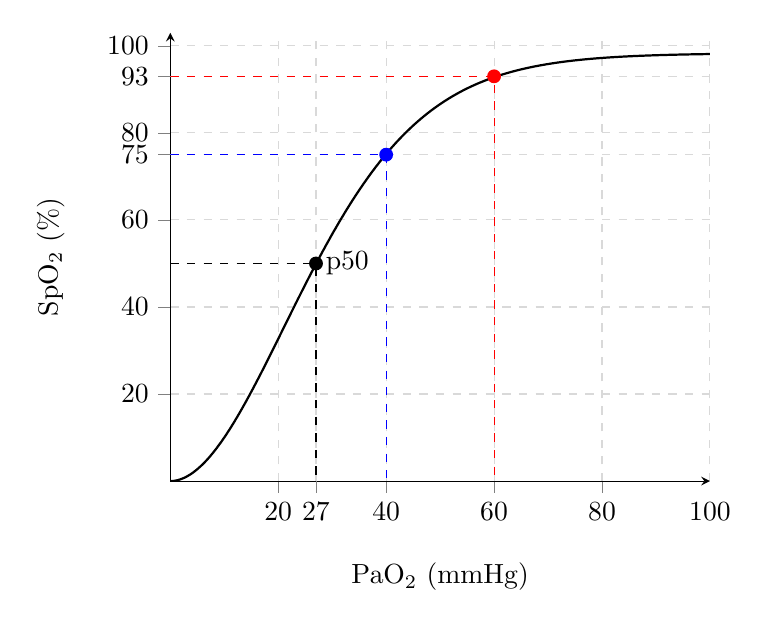
\begin{tikzpicture}

\tikzset{
    myarrow/.style={
        sloped,
        isosceles triangle,
        anchor=apex,
        fill=black,
        inner sep=2pt
    }
}

\makeatletter
\def\parsenode[#1]#2\pgf@nil{%
    \tikzset{label node/.style={#1}}
    \def\nodetext{#2}
}

\tikzset{
    add node at x/.style 2 args={
        name path global=plot line,
        /pgfplots/execute at end plot visualization/.append={
                \begingroup
                \@ifnextchar[{\parsenode}{\parsenode[]}#2\pgf@nil
            \path [name path global = position line #1-1]
                ({axis cs:#1,0}|-{rel axis cs:0,0}) --
                ({axis cs:#1,0}|-{rel axis cs:0,1});
            \path [xshift=1pt, name path global = position line #1-2]
                ({axis cs:#1,0}|-{rel axis cs:0,0}) --
                ({axis cs:#1,0}|-{rel axis cs:0,1});
            \path [
                name intersections={
                    of={plot line and position line #1-1},
                    name=left intersection
                },
                name intersections={
                    of={plot line and position line #1-2},
                    name=right intersection
                },
                label node/.append style={pos=1}
            ] (left intersection-1) -- (right intersection-1)
            node [label node]{\nodetext};
            \endgroup
        }
    },
    add node at y/.style 2 args={
        name path global=plot line,
        /pgfplots/execute at end plot visualization/.append={
                \begingroup
                \@ifnextchar[{\parsenode}{\parsenode[]}#2\pgf@nil
            \path [name path global = position line #1-1]
                ({axis cs:0,#1}-|{rel axis cs:0,0}) --
                ({axis cs:0,#1}-|{rel axis cs:1,1});
            \path [yshift=1pt, name path global = position line #1-2]
                ({axis cs:0,#1}-|{rel axis cs:0,0}) --
                ({axis cs:0,#1}-|{rel axis cs:1,1});
            \path [
                name intersections={
                    of={plot line and position line #1-1},
                    name=left intersection
                },
                name intersections={
                    of={plot line and position line #1-2},
                    name=right intersection
                },
                label node/.append style={pos=1}
            ] (left intersection-1) -- (right intersection-1)
            node [label node] {\nodetext};
            \endgroup
        }
    }
}
\makeatother
    \begin{axis}[
        axis lines=middle,
	ymin = 0,
	ymax = 103,
	xmin = 0,
xmax = 100,
        grid = major,
        grid style={dashed, gray!30},
	 ylabel near ticks,
	xlabel near ticks,
		extra x ticks={27},
	extra x tick labels = {27},
		extra y ticks={75,93},
	extra y tick labels = {75,93},
        xlabel=PaO\textsubscript{2} (mmHg),
        ylabel=SpO\textsubscript{2} (\%),
        tick align=outside,
        enlargelimits=false]

	\addplot[domain=0:100, black, thick,samples=500] {98.32157 + (-0.008578349 - 98.32157)/(1 + (x/90.23375)^1.937563)^7.691635};

\draw [black, thin, dashed] (0,50)-- (27, 50) node[circle,fill=black,inner sep=0pt,minimum size=5pt](p50){} node[right](){p50}-- (27, 0);
\draw [blue, thin, dashed] (0,75)-- (40, 75)  node[circle,fill=blue,inner sep=0pt,minimum size=5pt](){} -- (40, 0);
\draw [red, thin, dashed] (0,93)-- (60, 93)  node[circle,fill=red,inner sep=0pt,minimum size=5pt](p50){} -- (60, 0);
\end{axis}

\end{tikzpicture} 
\end{document}